%%%%%%%%%%%%%%%%%%%%%%%%%%%%%%%%%%%%%%%%%%%%%%%%
% E.Pinault-Bigeard - s2i@pinault-bigeard.com
% http://s2i.pinault-bigeard.com
% CC BY-NC-SA 2.0 FR - http://creativecommons.org/licenses/by-nc-sa/2.0/fr/
%%%%%%%%%%%%%%%%%%%%%%%%%%%%%%%%%%%%%%%%%%%%%%%%
\documentclass[11pt]{article}

%%%%%%%%%%%%%%%%%%%%%%%%%%%%%%%%%%%%%%%%%%%%%%%%
% Package UPSTI_Document
%%%%%%%%%%%%%%%%%%%%%%%%%%%%%%%%%%%%%%%%%%%%%%%% 
\RequirePackage[kholle]{UPSTI_Document}

%---------------------------------%
% Paramètres du package
%---------------------------------%

% Version du document (pour la compilation)
% 1: Document prof
% 2: Document élève
% 3: Document à publier
\newcommand{\UPSTIidVersionDocument}{1}

% Choix du type de document
% 4: Colle
\newcommand{\UPSTIidTypeDocument}{4}

% Titre principal
\newcommand{\UPSTItitreEnTete}{Dynamique}
\newcommand{\UPSTItitre}{Chaises volantes}      

% Source
\newcommand{\UPSTIsource}{E. NERKOWSKI}

% Versioning
\newcommand{\UPSTInumeroVersion}{1.0}
                 
%----------------------------------------------- 
\UPSTIcompileVars		% "Compile" les variables
%%%%%%%%%%%%%%%%%%%%%%%%%%%%%%%%%%%%%%%%%%%%%%%% 


%%%%%%%%%%%%%%%%%%%%%%%%%%%%%%%%%%%%%%%%%%%%%%%% 
% Début du document
%%%%%%%%%%%%%%%%%%%%%%%%%%%%%%%%%%%%%%%%%%%%%%%% 
\begin{document}

% Création de l'en-tête
\UPSTIbuildPage 

\section{Présentation}
\begin{wrapfigure}{r}{4cm}
  \centering
  \vspace{-2em}
  \fbox{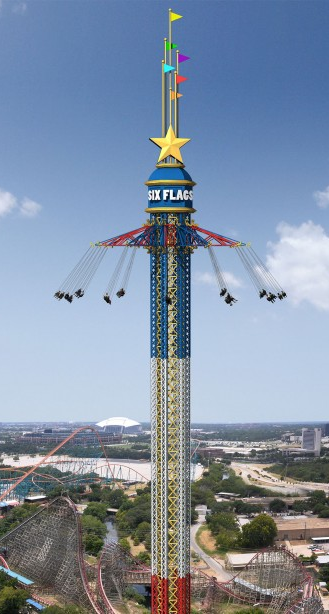
\includegraphics[width=3.5cm]{Src/Images/photo.png}}
  \vspace{-8em}
\end{wrapfigure}
Un manège est constitué d'un socle \np{1}, d'un fût central \np{2} qui supporte dix potences. Au bout de chacune d'elles, est suspendu l'ensemble noté \np{3} constitué d'une barre et du passager. Le siège est situé en $B$ et fait partie intégrante de cet ensemble \np{3} rigide. La direction \vz1 est verticale. Les liaisons sont parfaites et sans frottement.

On donne :
\begin{itemize}
\item $\vecteur{O_1A}=R\cdot\vx2$ \qquad $\vecteur{AG_3}=-L\cdot\vz3$ \qquad $\vy2=\vy2'=\vy3$
\item Solide \np{3}: masse $m_3$, centre d'inertie $G_3$, $\operateurInertie{A}{3}=\matriceInertie[b_3][A_3][B_3][C_3]$
\item La schématisation cinématique:
\end{itemize}

\begin{figure}[!ht]
    \centering
	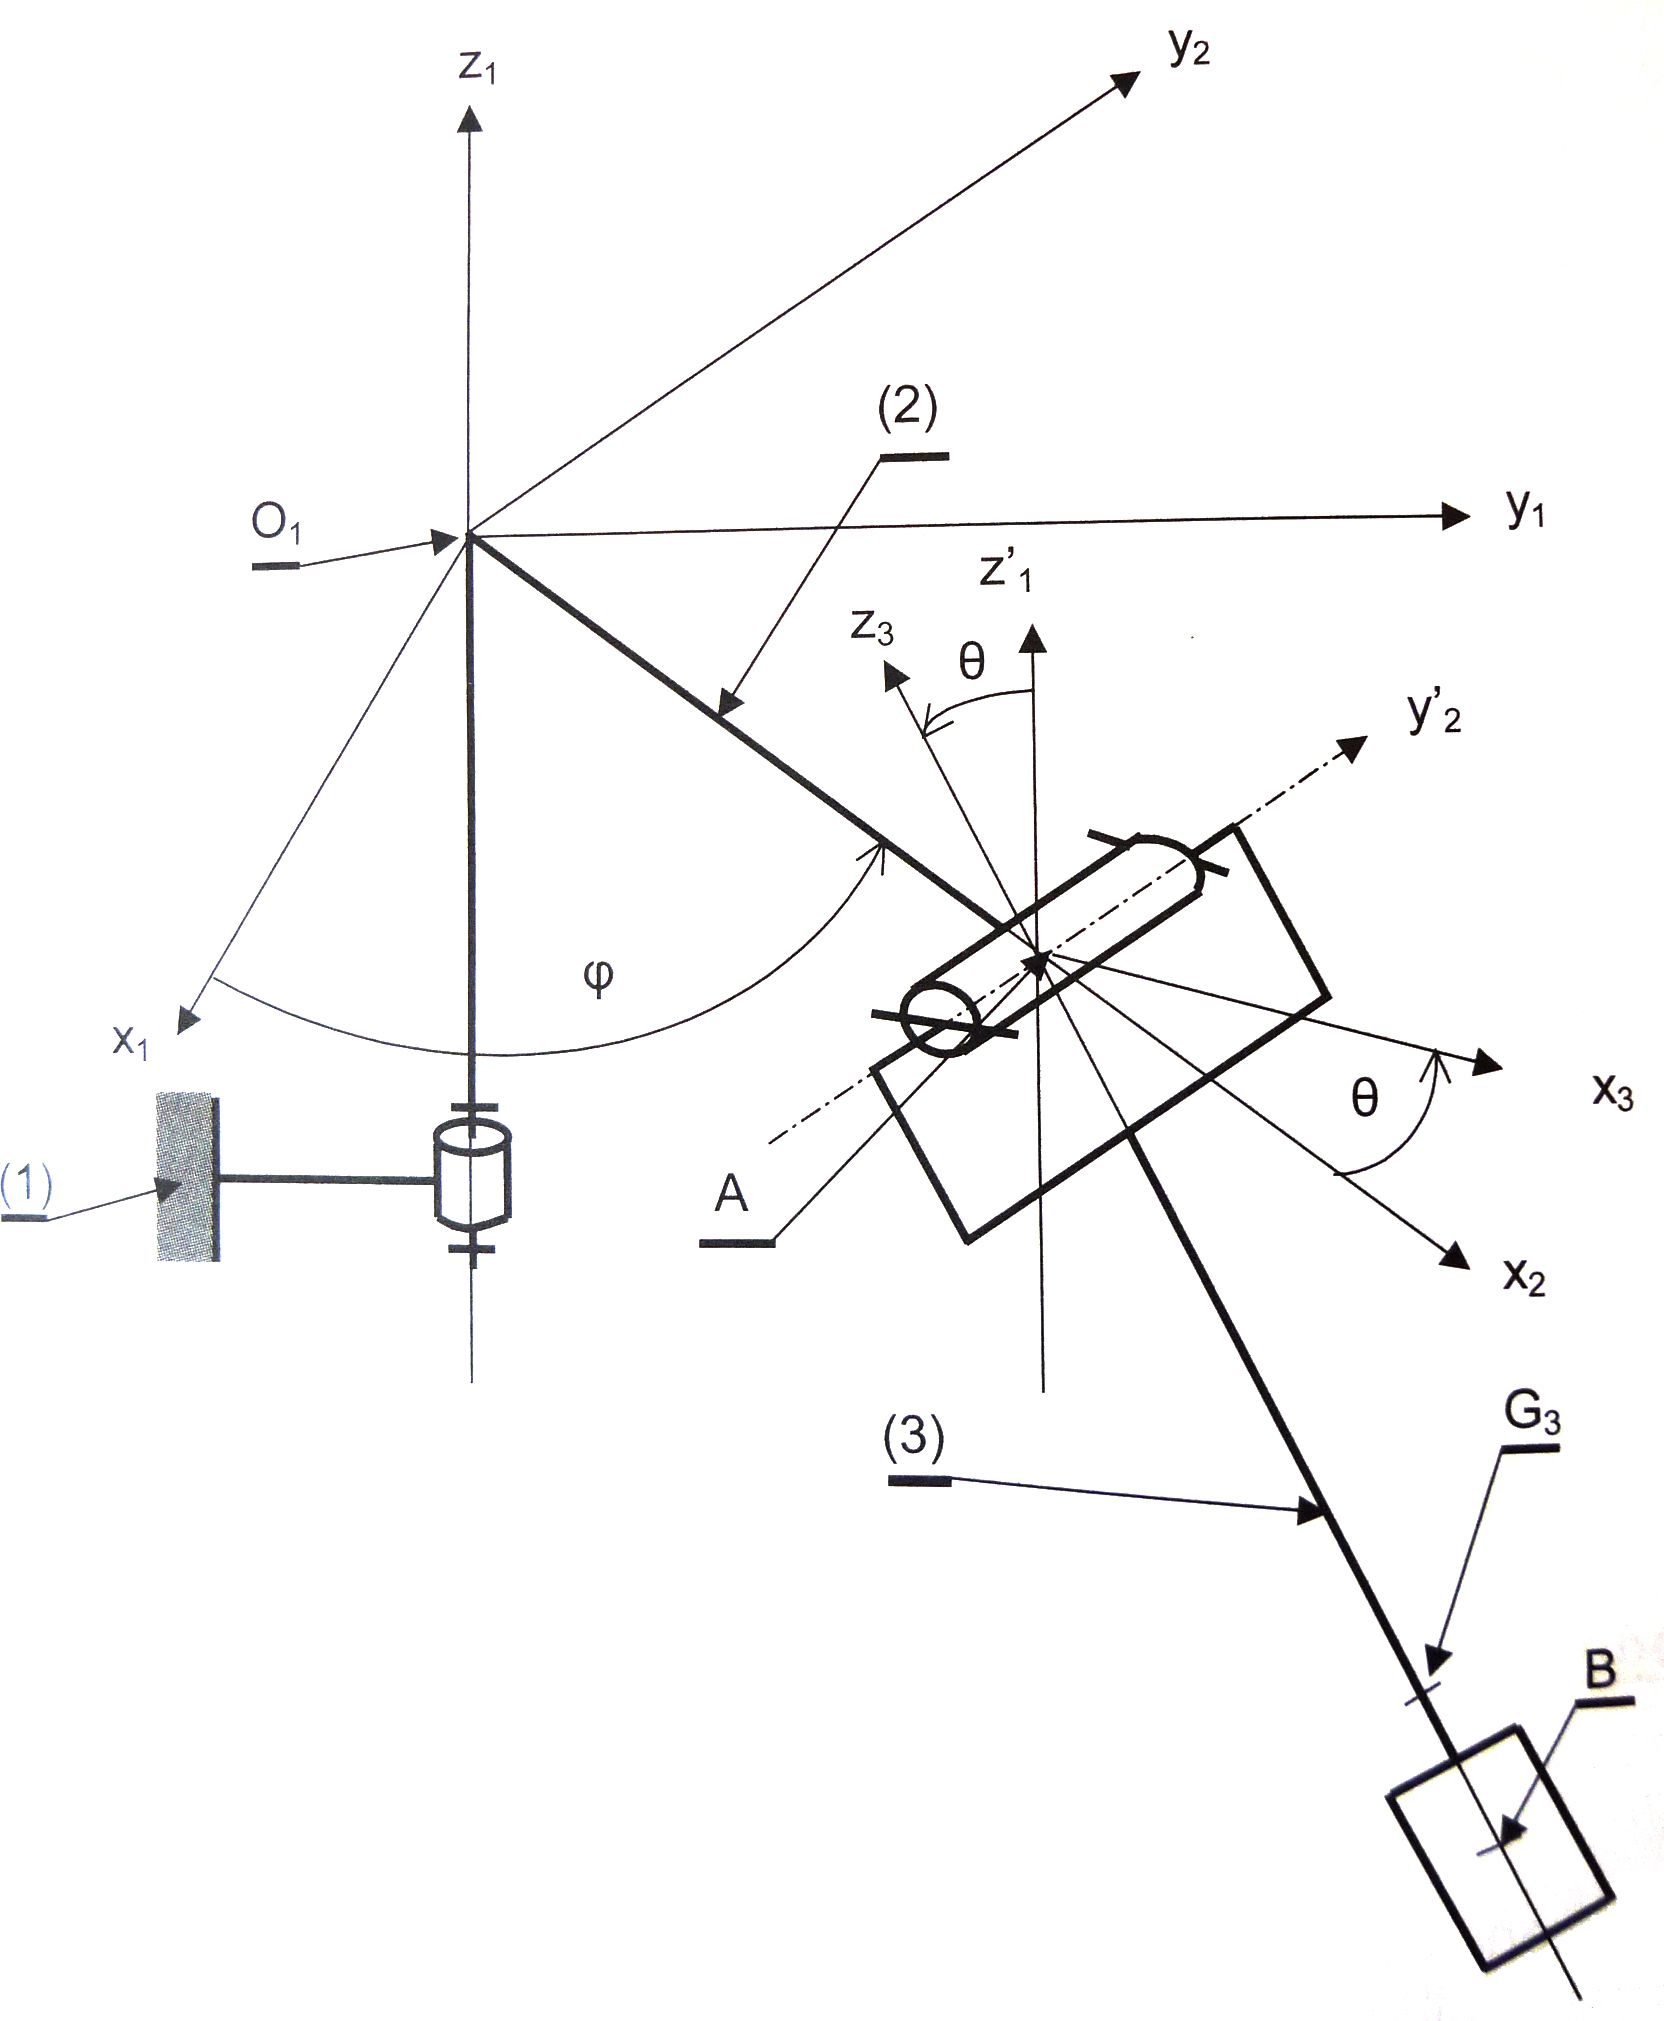
\includegraphics[width=9cm]{Src/Images/sc.jpg}
\end{figure}

\UPSTIobjectif{
L'objectif est de déterminer l'angle d'inclinaison $\theta$ correspondant à une vitesse de rotation du manège donnée.}

\section{Travail demandé}
\UPSTIquestion{Tracer le graphe des liaisons en plaçant l'ensemble des informations nécessaires à l'étude.}

\UPSTIcorrection{
\vspace{-2em}
\begin{center}
\begin{grapheLiaisons}[scale=0.7]
\glBati[-90]{0,0}{P1}{1}[1/0.7]
\glPiece{4,1}{P2}{2}
\glPiece{8,0}{P3}{3}
\glLiaison[bend left=10]{P1}{P2}[Pivot\\ axe \axe{O_1}{\vz1}][above]
\glLiaison[bend left=10]{P2}{P3}[Pivot\\ axe \axe{A}{\vy2}][above]
\draw[UPSTIcustomColor1,>=latex,<-,double] (P2) to[bend right] ++(1,-1.5) node[right] {\tAM{\mot}{2}};
\draw[UPSTIcustomColor1,>=latex,<-] (P3.300) to[bend right] ++(1.2,-0.5) node[right] {\tAM{\pes}{3}};
\end{grapheLiaisons}
\end{center}
\vspace{-2em}
}

\UPSTIquestion{Réaliser les figures de changement de bases.}

\UPSTIcorrection{
\vspace{-2em}
\begin{center}
\setCouleursParametrage{black}{UPSTIcustomColor1}
\parametrageAngulaire{\varphi}{\vx1}{\vy1}{\vz1}{\vx2}{\vy2}[\vz2]\qquad
\setCouleursParametrage{UPSTIcustomColor1}{UPSTIcustomColor3}
\parametrageAngulaire{\theta}{\vz2}{\vx2}{\vy2}{\vz3}{\vx3}[\vy3]
\end{center}
\vspace{-1em}
}

\UPSTIquestion{Préciser le torseur des actions mécaniques de \np{2} sur \np{3} en $A$ dans la
base $b_2$.}

\UPSTIcorrection{Liaison pivot d'axe \axe{A}{\vy2}:\quad $\UPSTIcadreMathCor{\tAM{2}{3}=\tCan{A}{\tActionMecaniqueCan{A}{2}{3}{1}{1}{1}{1}{0}{1}}{\bB2}}$}

\UPSTIquestion{Déterminer la stratégie d'isolement et de projection afin d'étudier les variations de l'angle $\theta$.}

\UPSTIcorrection{On isole \np{3} puis on applique le théorème du moment dynamique en $A$ autour de $\vy2=\vy3$. Comme cela, on trouvera directement l'équation du mouvement et on ne verra pas apparaitre les actions mécaniques de la liaison pivot.}

\UPSTIeleveOnly{\vspace{1em}}
La vitesse de rotation $\varphip$ est constante. De plus, on suppose que le moment d'inertie $C_3$ est négligeable devant les autres.

\UPSTIquestion{Déterminer le torseur cinétique en $A$ de \np{3} dans $\rR1$.}

\UPSTIcorrection{
\UPSTItitreStd{Résultante cinétique}
$\vVitesse{G_3}{3}{1}=\derivV{\vecteur{O_1G_3}}{\rR1}=\derivVl{R.\vx2-L.\vz3}{\rR1}$

Avec:\quad $\derivV{\vx2}{\rR1}=\varphip.\vy2$\quad et\quad $\derivV{\vz3}{\rR1}=-\thetap.\vx3-\varphip\sin\theta.\vy2$

On a alors:\quad $\vVitesse{G_3}{3}{1}=-L\thetap.\vx3+(R-L\sin\theta)\varphip.\vy2$

Soit enfin:\quad $\Res{\tC{3}{1}}=\resultanteCinetique[m_3][G_3]{3}{1}=\UPSTIcadreMathCor{m_3\left(-L\thetap.\vx3+(R-L\sin\theta)\varphip.\vy2\right)}$

\UPSTItitreStd[1]{Moment cinétique en $A$}
$\Mom{A}{\tC{3}{1}}=\momentCinetique{A}{3}{1}=\operateurInertie{A}{3}.\vRotation{3}{1}+m_3\vecteur{AG_3}\vect\vVitesse{A}{3}{1}$

Pour le produit matriciel, il faut exprimer $\vRotation{3}{1}$ dans \bB3:\quad $\vRotation{3}{1}=\thetap.\vy3+\varphip.\vz1=\vColonne{-\varphip\sin\theta\\ \thetap\\ \varphip\cos\theta}[\bB3]$

Soit, avec $C_3$ négligeable:\quad $\operateurInertie{A}{3}.\vRotation{3}{1}=-A_3\varphip\sin\theta.\vx3+B_3\thetap.\vy3$

Et:\quad $\vecteur{AG_3}\vect\vVitesse{A}{3}{1}=-L.\vz3\vect R\varphip.\vy2=LR\varphip.\vx3\quad\Rightarrow\quad \momentCinetique{A}{3}{1}=\UPSTIcadreMathCor{\left(m_3LR-A_3\sin\theta\right)\varphip.\vx3+B_3\thetap.\vy3}$

\UPSTItitreStd[1]{Torseur cinétique}
En combinant les 2 résultats précédents:\quad $\UPSTIcadreMathCor{\tC{3}{1}=\tLigne{A}{m_3\left(-L\thetap.\vx3+(R-L\sin\theta)\varphip.\vy2\right)}{\left(m_3LR-A_3\sin\theta\right)\varphip.\vx3+B_3\thetap.\vy3}}$
}

\UPSTIquestion{Déterminer le torseur dynamique en $A$ de \np{3} dans $\rR1$.}

\UPSTIcorrection{
\UPSTItitreStd{Résultante dynamique}
$\vAcceleration{G_3}{3}{1}=\derivVl{\vVitesse{G_3}{3}{1}}{\rR1}$\quad avec:\quad $\derivV{\vx3}{\rR1}=-\thetap.\vz3+\varphip\cos\theta.\vy3$

Alors:\quad $\Res{\tD{3}{1}}=\resultanteDynamique[m_3][G_3]{3}{1}=\UPSTIcadreMathCor{m_3\left(-L\thetapp.\vx3-2L\thetap\varphip\cos\theta.\vy2-(R-L\sin\theta)\varphip^2.\vx2+L\thetap^2.\vz3\right)}$

\UPSTItitreStd[1]{Moment dynamique en $A$}

On a:\quad $\Mom{A}{\tD{3}{1}}=\momentDynamique{A}{3}{1}=\derivVl{\momentCinetique{A}{3}{1}}{\rR1}+\vVitesse{A}{}{1}\vect \resultanteCinetique[m_3][G_3]{3}{1}$\quad ce qui donne après calculs:

$\UPSTIcadreMathCor{\momentDynamique{A}{3}{1}=-B_3\varphip\thetap.\vx2-A_3\varphip\thetap\cos\theta.\vx3+\left(\left(-A_3\sin\theta+m_3LR\right)\varphip^2\cos\theta+B_3\thetapp\right).\vy2+A_3\sin\theta\varphip\thetap.\vz3}$

\UPSTItitreStd[1]{Torseur dynamique}
En combinant les 2 résultats précédents:

$\UPSTIcadreMathCor{\tD{3}{1}=\tLigne{A}{m_3\left(-L\thetapp.\vx3-2L\thetap\varphip\cos\theta.\vy2-(R-L\sin\theta)\varphip^2.\vx2+L\thetap^2.\vz3\right)}{-B_3\varphip\thetap.\vx2-A_3\varphip\thetap\cos\theta.\vx3+\left(\left(-A_3\sin\theta+m_3LR\right)\varphip^2\cos\theta+B_3\thetapp\right).\vy2+A_3\sin\theta\varphip\thetap.\vz3}}$}

\UPSTIquestion{Déterminer l'équation différentielle qui gouverne les variations de l'angle $\theta$.}

\UPSTIcorrection{
On va appliquer le PFD à \np{3} et on écrira l'équation de moment en $A$ en projection sur $\vy2$. De cette manière, on ne verra pas apparaître les inconnues de liaison de la liaison pivot.

\UPSTItitreStd{IAME}
\begin{itemize}
\item $Mom{A}{\tAM{\pes}{3}}\cdot\vy2=-Lm_3g\sin\theta$
\end{itemize}

\UPSTItitreStd{PFD}
En reprenant les résultats précédents, on trouve:\quad $\UPSTIcadreMathCor{B_3\thetapp+\varphip^2\cos\theta\left(m_3LR-A_3\sin\theta\right)=-Lm_3g\sin\theta}$\quad (1)
}

\UPSTIeleveOnly{\vspace{1em}}
A une vitesse de rotation constante, la barre \np{3} se stabilise par rapport à \np{2} : $\theta$ est alors constant et noté $\theta_s$.

\UPSTIquestion{Déterminer l'expression de cet angle d'inclinaison en supposant qu'en première approximation $A_3$ peut être négligé devant le produit $m_3LR$. Réaliser l'application numérique avec $R=\SI{4}{m}$ et $\varphip=\SI{1}{rad.s^{-1}}$.}

\UPSTIcorrection{Avec $\theta=\theta_s$ et $A_3\ll m_3LR$:\quad $(1): m_3LR\varphip^2=-Lm_3g\sin\theta\quad\Rightarrow\quad\UPSTIcadreMathCor{\tan\theta_s=-\dfrac{R\varphip^2}{g}}$

\noindent \AN\quad $\UPSTIcadreMathCor{\theta_s=\SI{-22,2}{\degree}}$\quad ($<0$ car attiré vers l'extérieur... comportement logique)
}

\UPSTIquestion{Déterminer dans ce cas l'expression des composantes de \tAM{2}{3}.}

\UPSTIcorrection{On reprend le PFD appliqué à \np{3}:\quad $\UPSTIcadreMathCor{\tAM{2}{3}=\tColonne{A}{-m_3\left(R-L\sin\theta\right)\varphip^2 \\ 0 \\m_3g}{0\\0\\0}{\bB2}}$}

\UPSTIquestion{Réaliser l'application numérique avec: $L=\SI{2}{m}$ \quad $m_3=\SI{100}{kg}$ \quad $A_3=B_3=\SI{130}{kg.m^2}$.}

\UPSTIcorrection{$\tAM{2}{3}=\tColonne{A}{-324 \\ 0 \\ 981}{0\\0\\0}{\bB2}\quad\Rightarrow\quad \UPSTIcadreMathCor{\norme{\resultanteAM{2}{3}}=\SI{1033}{N}}$
}

\UPSTIquestion{Dessiner dans le plan \triplet{A_2}{\vx2}{\vz1} la position de la barre ainsi que les efforts qu'elle subit.}

\UPSTIcorrection{
\vspace{-1em}
\begin{figure}[!ht]
    \centering
	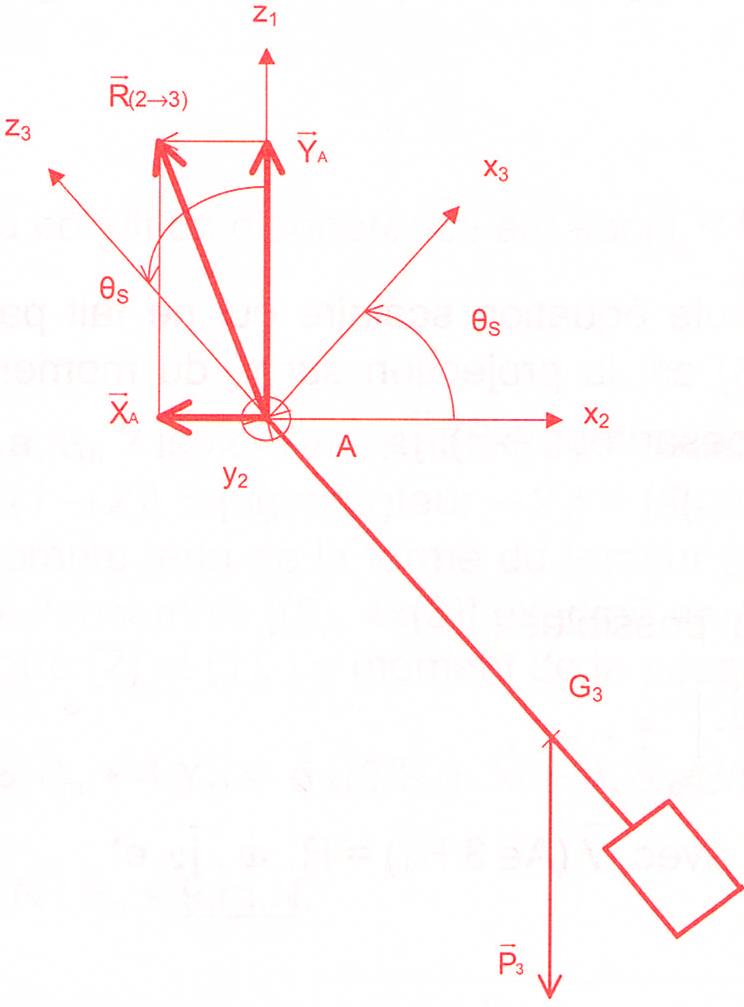
\includegraphics[width=8cm]{Src/Images/corrige.png}
\end{figure}
}

\end{document}
